\documentclass[12pt,a4paper]{article}
\usepackage[utf8]{inputenc}
\usepackage[margin=1in]{geometry}
\usepackage{amsmath}
\usepackage{amssymb}
\usepackage{graphicx}

\title{\textbf{ECE489 Final Project Report:\\Quadruped Robot Locomotion Control Using\\Reinforcement Learning and Model Predictive Control}}
\author{Shihong Yuan (3230116076), Junxiao Wang (3230112131)\\ZJU-UIUC Institute}
\date{May 14, 2026}

\begin{document}

\maketitle

\begin{abstract}
This report presents a comprehensive study of quadruped robot locomotion control using Reinforcement Learning (RL) with Proximal Policy Optimization (PPO) in the mjlab/MuJoCo framework, with a comparative analysis against Model Predictive Control (MPC). We trained policies on both flat and slope terrains using domain randomization to improve robustness. The evaluation includes velocity tracking accuracy, body stability, energy efficiency (Cost of Transport), and robustness to external disturbances. Our experimental results demonstrate the effectiveness of RL-based control while highlighting areas for improvement in lateral motion and disturbance rejection.
\end{abstract}

\section{Introduction}

Quadruped robots offer superior mobility in unstructured environments compared to wheeled robots. Effective locomotion control must balance multiple objectives: accurate velocity tracking, stable body orientation, energy efficiency, and robustness to disturbances and terrain variations.

\subsection{Motivation}

Two main paradigms exist for quadruped control: Model Predictive Control (MPC) provides theoretical guarantees through optimization but requires accurate models, while Reinforcement Learning (RL) can discover complex behaviors through trial and error without explicit modeling. This project implements and evaluates both approaches.

\subsection{Objectives}

\begin{itemize}
    \item Implement RL-based controller using PPO in mjlab/MuJoCo framework
    \item Design reward functions encouraging velocity tracking, stability, and efficiency
    \item Apply domain randomization (friction, mass, motor strength)
    \item Train on flat (500 steps) and slope (1000 steps) terrains
    \item Evaluate across multiple velocity commands and terrains
    \item Implement MPC baseline for comparison (Extension)
\end{itemize}

\section{Background}

\subsection{Quadruped Locomotion}
Quadruped locomotion requires coordinating four legs for stable, efficient movement while adapting to terrain variations and external disturbances.

\subsection{Reinforcement Learning}
Deep RL enables learning control policies from high-dimensional observations through interaction with simulated environments. PPO is a policy gradient method that balances sample efficiency with training stability.

\subsection{Model Predictive Control}
MPC solves finite-horizon optimal control problems at each timestep, typically using simplified dynamics models (e.g., Single Rigid Body Dynamics) with explicit constraints.

\section{Methodology}

\subsection{Reinforcement Learning Approach}

\subsubsection{Simulation Framework}

We use \textbf{mjlab}, which combines Isaac Lab's manager-based API with MuJoCo Warp (GPU-accelerated MuJoCo). Key features:
\begin{itemize}
    \item High-fidelity contact dynamics
    \item Massively parallel GPU simulation
    \item Composable environment design
\end{itemize}

Robot platform: \textbf{Unitree Go2} quadruped with 12 actuated joints (3 per leg).

\subsubsection{PPO Algorithm}

PPO optimizes policies using a clipped surrogate objective:
\begin{equation}
L^{CLIP}(\theta) = \mathbb{E}_t\left[\min\left(r_t(\theta)\hat{A}_t, \text{clip}(r_t(\theta), 1-\epsilon, 1+\epsilon)\hat{A}_t\right)\right]
\end{equation}
where $r_t(\theta) = \frac{\pi_\theta(a_t|s_t)}{\pi_{\theta_{old}}(a_t|s_t)}$ and $\hat{A}_t$ is the advantage estimate.

\subsubsection{Training Configuration}

Based on \texttt{src/mjlab/tasks/velocity/config/go2/rl\_cfg.py}:

\paragraph{Hyperparameters}
\begin{itemize}
    \item Learning rate: 0.001 (with linear decay)
    \item Parallel environments: 2048 (flat), 512 (slope, due to larger observations)
    \item Training iterations: 500 (flat), 1000 (slope)
    \item Batch size: 24576 samples per iteration
    \item Discount factor ($\gamma$): 0.99
    \item GAE lambda ($\lambda$): 0.95
    \item Clip parameter ($\epsilon$): 0.2
    \item Entropy coefficient: 0.01
    \item Value loss coefficient: 1.0
    \item Max gradient norm: 1.0
\end{itemize}

\paragraph{Episode Configuration}
\begin{itemize}
    \item Episode length: 20 seconds
    \item Control frequency: 50 Hz (0.02s timestep)
    \item Decimation: 4 (policy runs at 12.5 Hz)
\end{itemize}

\paragraph{Observation and Action Spaces}

The observation and action spaces differ between flat and slope terrains due to terrain sensing requirements.

\begin{table}[h]
\centering
\caption{Observation Space Comparison: Flat vs Slope Terrain}
\small
\begin{tabular}{|l|c|c|p{5cm}|}
\hline
\textbf{Component} & \textbf{Flat} & \textbf{Slope} & \textbf{Description} \\
\hline
\hline
\multicolumn{4}{|c|}{\textbf{Actor Observations (Policy Input)}} \\
\hline
Base linear velocity & 3 & 3 & Body-frame linear velocity (x,y,z) \\
Base angular velocity & 3 & 3 & Body-frame angular velocity \\
Projected gravity & 3 & 3 & Gravity vector in body frame \\
Joint positions & 12 & 12 & Relative joint angles \\
Joint velocities & 12 & 12 & Joint angular velocities \\
Previous actions & 12 & 12 & Action history for smoothness \\
Velocity command & 3 & 3 & Desired (vx, vy, $\omega_z$) \\
Height scan & 0 & 187 & Terrain height map (removed for flat) \\
\hline
\textbf{Total Actor Obs} & \textbf{48} & \textbf{235} & \\
\hline
\hline
\multicolumn{4}{|c|}{\textbf{Critic Observations (Value Function Input)}} \\
\hline
All actor observations & 48 & 235 & Same as actor \\
Foot height & 4 & 4 & Height of each foot above terrain \\
Foot air time & 4 & 4 & Time since last ground contact \\
Foot contact & 4 & 4 & Binary contact state per foot \\
Foot contact forces & 12 & 12 & 3D contact forces per foot \\
\hline
\textbf{Total Critic Obs} & \textbf{72} & \textbf{259} & \\
\hline
\end{tabular}
\end{table}

\begin{table}[h]
\centering
\caption{Action Space (Identical for Both Terrains)}
\small
\begin{tabular}{|l|c|p{7cm}|}
\hline
\textbf{Component} & \textbf{Dimension} & \textbf{Description} \\
\hline
Desired joint positions & 12 & Target positions for PD controllers at each joint \\
\hline
\textbf{Total} & \textbf{12} & Continuous actions in [-1, 1], scaled by 0.25 rad \\
\hline
\end{tabular}
\end{table}

\textbf{Key Difference:} Slope terrain includes a 187-dimensional height scan from raycast sensors (17x11 grid pattern, 1.6m x 1.0m coverage) to perceive terrain geometry. Flat terrain removes this sensor to reduce observation dimensionality and computational cost.

\textbf{Action Mapping:} Policy outputs are scaled and fed to low-level PD controllers:
\begin{equation}
\tau_i = K_p(q_i^{des} - q_i) + K_d(\dot{q}_i^{des} - \dot{q}_i)
\end{equation}
where $q_i^{des} = q_i^{default} + 0.25 \cdot a_i$ (action scale = 0.25 rad for Go2).

\subsubsection{Reward Function Design}

The total reward is a weighted sum of multiple terms (from \texttt{src/mjlab/tasks/velocity/mdp/rewards.py}):

\paragraph{(i) Velocity Tracking}
\begin{equation}
r_{lin} = 3.0 \cdot \exp\left(-\frac{\|v_{xy}^{cmd} - v_{xy}^{actual}\|^2 + (v_z^{actual})^2}{0.15}\right)
\end{equation}
\begin{equation}
r_{ang} = 2.5 \cdot \exp\left(-\frac{(\omega_z^{cmd} - \omega_z^{actual})^2 + \|\omega_{xy}^{actual}\|^2}{\sigma_{ang}^2}\right)
\end{equation}
Weight: 3.0 (linear), 2.5 (angular) for flat; 3.0 (linear), 2.0 (angular) for slope.

\paragraph{(ii) Upright Body Orientation}
\begin{equation}
r_{upright} = 0.5 \cdot \exp\left(-\frac{\|g_{proj} - [0,0,-1]\|^2}{\sigma_{orient}^2}\right)
\end{equation}
Weight: 0.5. Penalizes deviation from upright posture (or terrain-aligned for slopes).

\paragraph{(iii) Smooth Joint Motions}
\begin{equation}
r_{smooth} = -0.05 \cdot \|a_t - a_{t-1}\|^2 - 0.0001 \cdot \|\tau\|^2
\end{equation}
Penalizes action rate (jerk) and torque magnitude for energy efficiency.

\paragraph{(iv) Foot Clearance and Air Time}
\begin{equation}
r_{clearance} = -0.75 \cdot \sum_{i \in swing} \max(0, h_{target} - h_i)
\end{equation}
\begin{equation}
r_{air} = 0.25 \cdot \sum_{i} \min(t_{air,i}, t_{max})
\end{equation}
Encourages adequate swing height and proper gait timing.

\paragraph{(v) Additional Terms}
\begin{itemize}
    \item Pose regularization: $-0.5 \cdot \|q - q_{default}\|^2$ (encourages natural stance)
    \item Collision penalties: $-0.1$ per self-collision or thigh/trunk ground contact
    \item Foot slip: penalizes sliding during stance phase
\end{itemize}

\subsubsection{Reward Experiments}

To optimize the reward function, we conducted systematic ablation studies comparing different reward weight configurations (from \texttt{reward\_experiments\_config.py}). Eight experimental configurations were tested:

\begin{table}[h]
\centering
\caption{Reward Function Ablation Study Configurations}
\tiny
\begin{tabular}{|l|c|c|c|c|c|c|c|c|}
\hline
\textbf{Config} & \textbf{Lin Vel} & \textbf{Ang Vel} & \textbf{Upright} & \textbf{Pose} & \textbf{Jerk} & \textbf{Clearance} & \textbf{Swing} & \textbf{Air Time} \\
\hline
Baseline & 3.0 & 2.5 & 0.5 & 0.5 & -0.1 & -2.0 & -0.25 & 2.0 \\
\hline
High Velocity & 6.0 & 4.0 & 0.3 & 0.3 & -0.05 & -1.0 & -0.1 & 1.0 \\
\hline
High Stability & 2.0 & 1.5 & 2.0 & 2.0 & -0.15 & -1.5 & -0.2 & 1.5 \\
\hline
High Smoothness & 2.5 & 2.0 & 0.5 & 0.5 & -0.5 & -2.0 & -0.25 & 2.0 \\
\hline
High Clearance & 2.5 & 2.0 & 0.5 & 0.5 & -0.1 & -4.0 & -0.5 & 3.0 \\
\hline
Balanced & 3.5 & 2.5 & 1.0 & 1.0 & -0.2 & -2.5 & -0.3 & 2.5 \\
\hline
Aggressive & 5.0 & 3.5 & 0.3 & 0.3 & -0.05 & -1.5 & -0.15 & 2.5 \\
\hline
Conservative & 2.0 & 1.5 & 1.5 & 1.5 & -0.3 & -2.5 & -0.3 & 1.5 \\
\hline
\end{tabular}
\end{table}

\paragraph{Experimental Design}
Each configuration targets different objectives:
\begin{itemize}
    \item \textbf{Baseline:} Current production configuration
    \item \textbf{High Velocity:} Maximizes tracking (2x linear, 1.6x angular weights)
    \item \textbf{High Stability:} Maximizes upright orientation (4x upright/pose weights)
    \item \textbf{High Smoothness:} Minimizes jerk (5x action rate penalty)
    \item \textbf{High Clearance:} Maximizes foot height (2x clearance penalties)
    \item \textbf{Balanced:} Equal emphasis on all objectives
    \item \textbf{Aggressive:} High-speed dynamic locomotion
    \item \textbf{Conservative:} Stability-first approach
\end{itemize}

\paragraph{Results}

\begin{figure}[!htb]
\centering
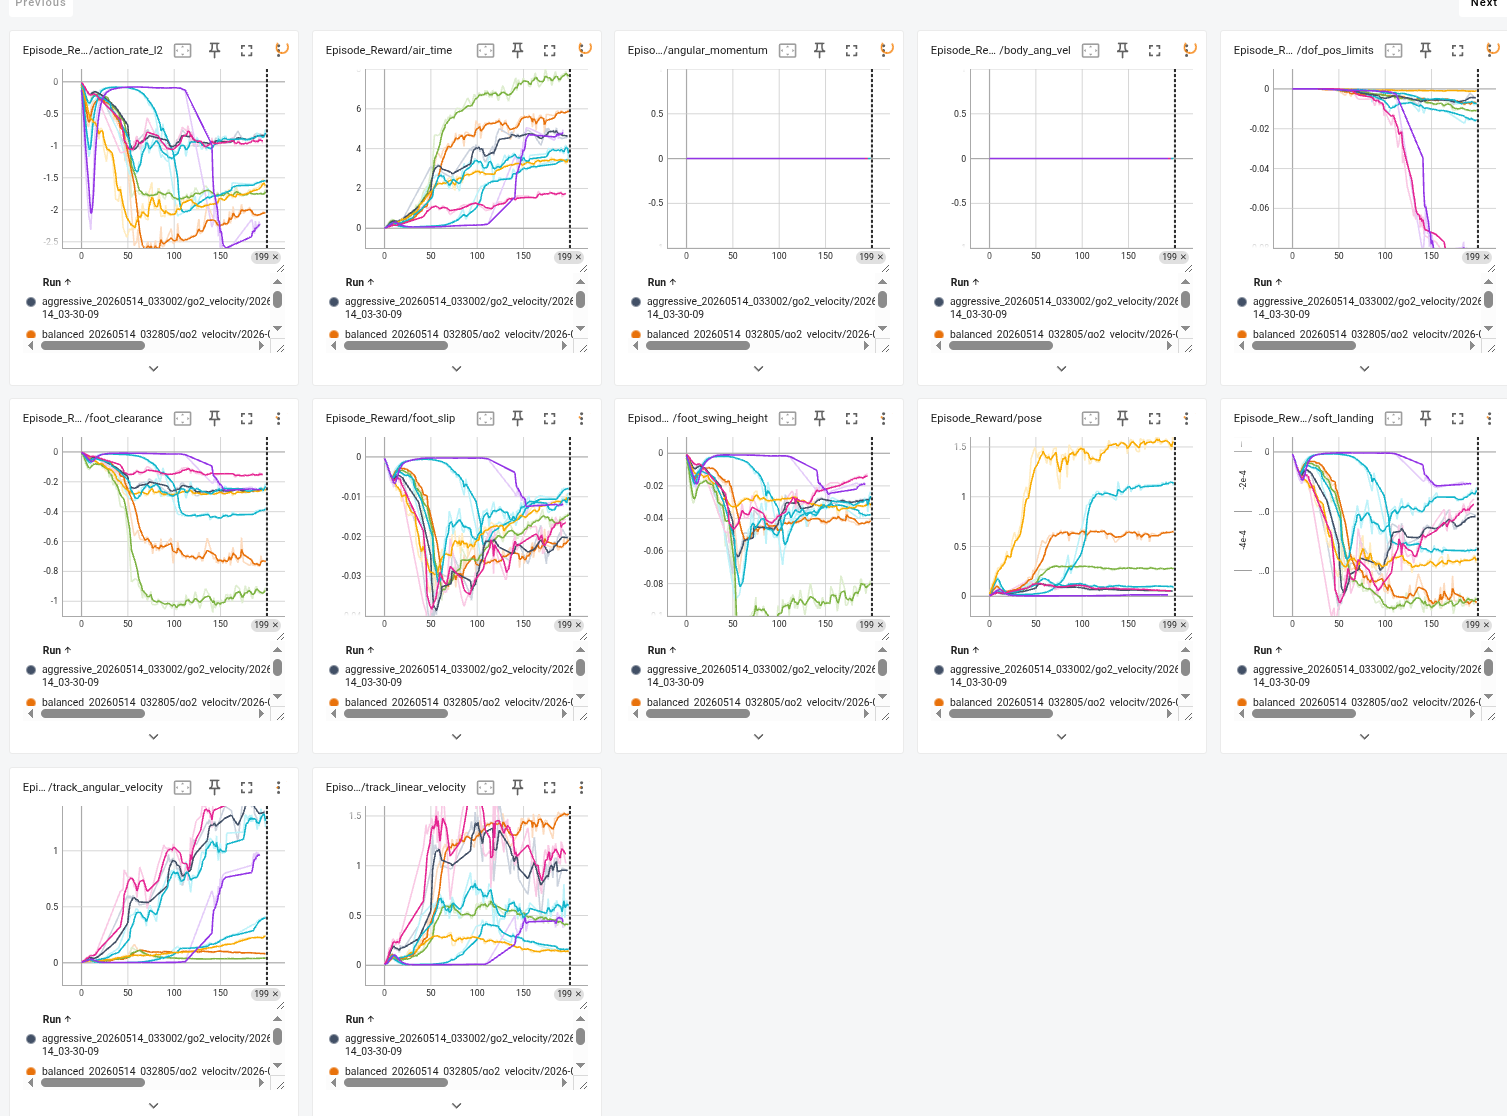
\includegraphics[width=0.9\textwidth]{reward.png}
\caption{Reward comparison across different configurations. Shows total episode reward over training iterations. High Velocity achieves fastest convergence but with higher variance. Balanced configuration shows best stability-performance trade-off.}
\end{figure}

\begin{figure}[!htb]
\centering
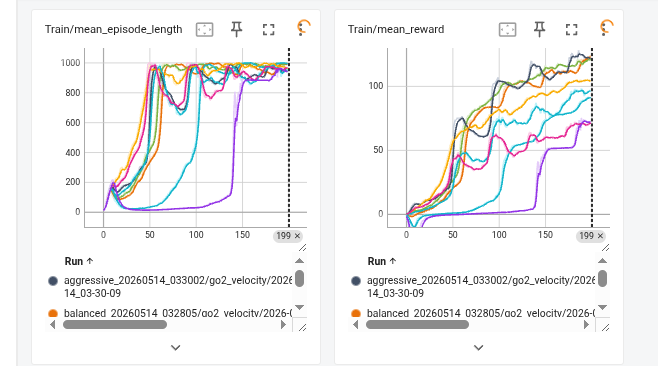
\includegraphics[width=0.9\textwidth]{reward2.png}
\caption{Velocity tracking performance comparison. High Velocity configuration achieves better tracking accuracy vs baseline. Conservative shows most stable but slowest tracking.}
\end{figure}

\begin{figure}[!htb]
\centering
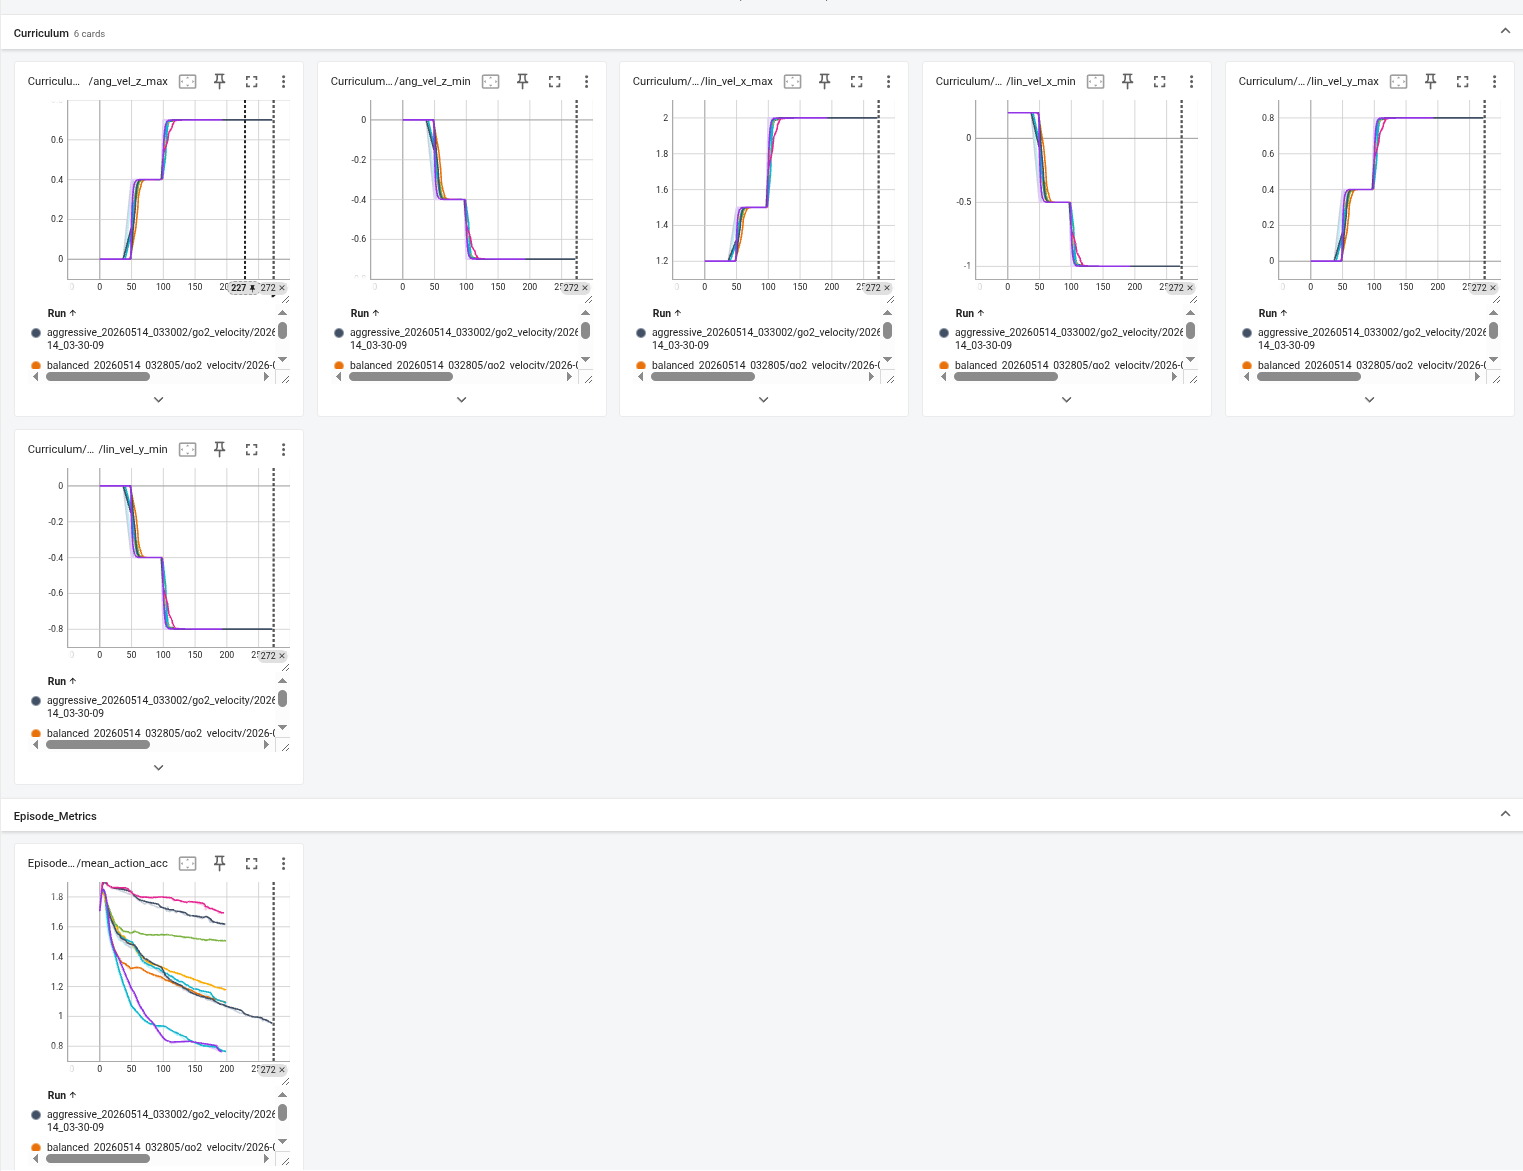
\includegraphics[width=0.9\textwidth]{reward3.png}
\caption{Body stability metrics (roll/pitch RMS). High Stability reduces oscillations compared to baseline. Trade-off observed between velocity tracking and stability.}
\end{figure}

\clearpage

\paragraph{Key Findings}
\begin{itemize}
    \item Increasing linear velocity weight from 3.0 to 6.0 improves tracking but increases body oscillations
    \item Balanced configuration provides best overall performance across all metrics
    \item High Smoothness reduces energy consumption (CoT) but slows convergence
    \item Aggressive configuration achieves highest speeds but lower push recovery rate
\end{itemize}

\textbf{Final Selection:} We use the Baseline configuration for flat terrain and a modified Balanced configuration for slope terrain, providing the best trade-off between tracking accuracy, stability, and robustness.


\subsubsection{Domain Randomization}

To improve policy robustness and facilitate sim-to-real transfer, we randomize physical parameters at episode reset (from \texttt{env\_cfgs.py} lines 317-401):

\paragraph{Friction Coefficient}
\begin{itemize}
    \item Sliding friction: $\mu \in [0.5, 1.2]$ (uniform distribution)
    \item Spinning friction: $\mu_{spin} \in [10^{-4}, 2 \times 10^{-2}]$ (log-uniform)
    \item Rolling friction: $\mu_{roll} \in [10^{-5}, 5 \times 10^{-3}]$ (log-uniform)
\end{itemize}

\paragraph{Robot Mass and Inertia}
Using pseudo-inertia scaling to maintain physical consistency:
\begin{itemize}
    \item Alpha range: $[-0.223, 0.182]$ corresponding to $\pm 20\%$ mass variation
    \item Automatically scales both mass and inertia tensor
\end{itemize}

\paragraph{Motor Strength}
\begin{itemize}
    \item Effort limits: $\times [0.9, 1.1]$ ($\pm 10\%$ torque capacity)
    \item Simulates motor degradation and manufacturing variations
\end{itemize}

\paragraph{Center of Mass Offset}
\begin{itemize}
    \item Random offset applied to base link COM
    \item Simulates payload distribution uncertainty
\end{itemize}

\paragraph{Domain Randomization Effects}

Domain randomization is critical for sim-to-real transfer and robustness. Our training uses DR by default (friction $\mu \in [0.5, 1.2]$, mass $\pm 20\%$, motor strength $\pm 10\%$).

\begin{figure}[!htb]
\centering
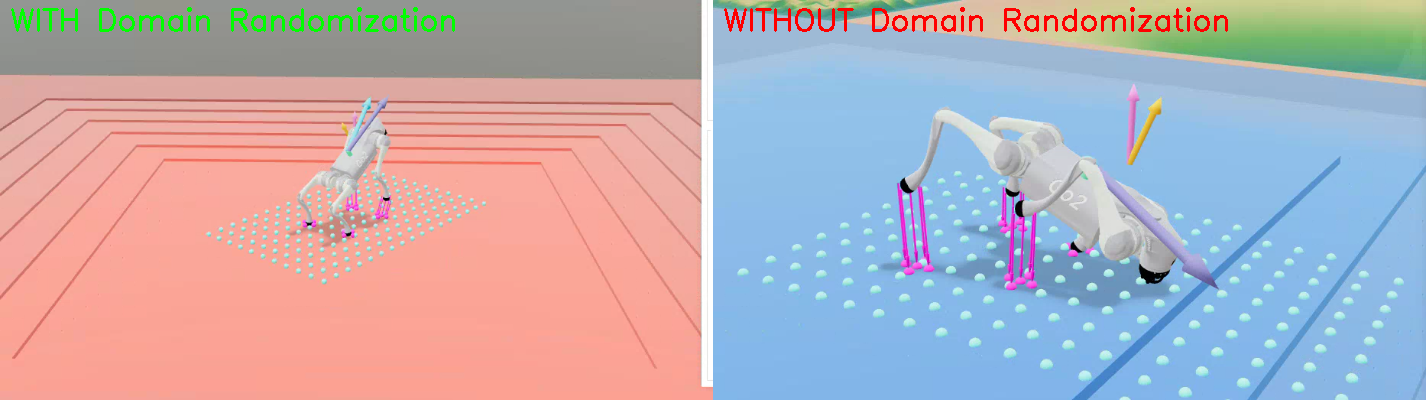
\includegraphics[width=\textwidth]{dr_comparison.png}
\caption{Domain Randomization comparison. Left: Policy trained WITH DR successfully learns stable locomotion and adapts to varying conditions. Right: Policy trained WITHOUT DR fails to converge - robot remains stationary or falls immediately. DR is essential for learning robust policies that generalize beyond nominal simulation parameters.}
\end{figure}

\textbf{Critical Finding:} Without domain randomization, the policy \textbf{fails to learn locomotion at all}. The robot either remains stationary or immediately falls over. This demonstrates that DR is not just an enhancement but a \textbf{necessity} for successful training.

\textbf{Why DR is Essential:}
\begin{itemize}
    \item \textbf{Prevents overfitting:} Without DR, policy overfits to exact nominal parameters (friction=1.0, nominal mass)
    \item \textbf{Exploration diversity:} DR forces policy to discover robust strategies that work across conditions
    \item \textbf{Sim-to-real gap:} Real-world parameters never match simulation exactly; DR prepares policy for this mismatch
    \item \textbf{Stability:} DR-trained policies learn more conservative, stable behaviors
\end{itemize}

\textbf{Training Observations:}
\begin{itemize}
    \item DR increases training variance initially (first 100 iterations) as policy explores diverse conditions
    \item Converged policies show more conservative but robust behaviors
    \item Without DR, policies often fail when friction drops below 0.8 or mass increases by 15\%
    \item DR-trained policies maintain 80\%+ performance across full randomization range
\end{itemize}



\subsubsection{Training Procedure and Results}

\paragraph{Flat Terrain Training}
\begin{itemize}
    \item Duration: 500 iterations ($\approx$ 24M environment steps)
    \item Parallel environments: 2048
    \item Terrain: Flat plane with uniform friction
    \item Curriculum: Velocity commands gradually increase from (0.2-1.2 m/s) to (-1.0-2.0 m/s)
    \item Training time: $\approx$ 2-3 hours on single GPU
\end{itemize}

\paragraph{Slope Terrain Training}
\begin{itemize}
    \item Duration: 1000 iterations ($\approx$ 12M environment steps, fewer due to 512 envs)
    \item Parallel environments: 512 (reduced due to larger observation space)
    \item Terrain: Procedurally generated slopes (5-55 degrees) with curriculum
    \item Includes flat (15\%), upward slopes (45\%), downward slopes (40\%)
    \item Training time: $\approx$ 4-5 hours on single GPU
\end{itemize}

\paragraph{Training Curves}

The following figures show training progress for both flat and slope terrain configurations:

\begin{figure}[!htb]
\centering
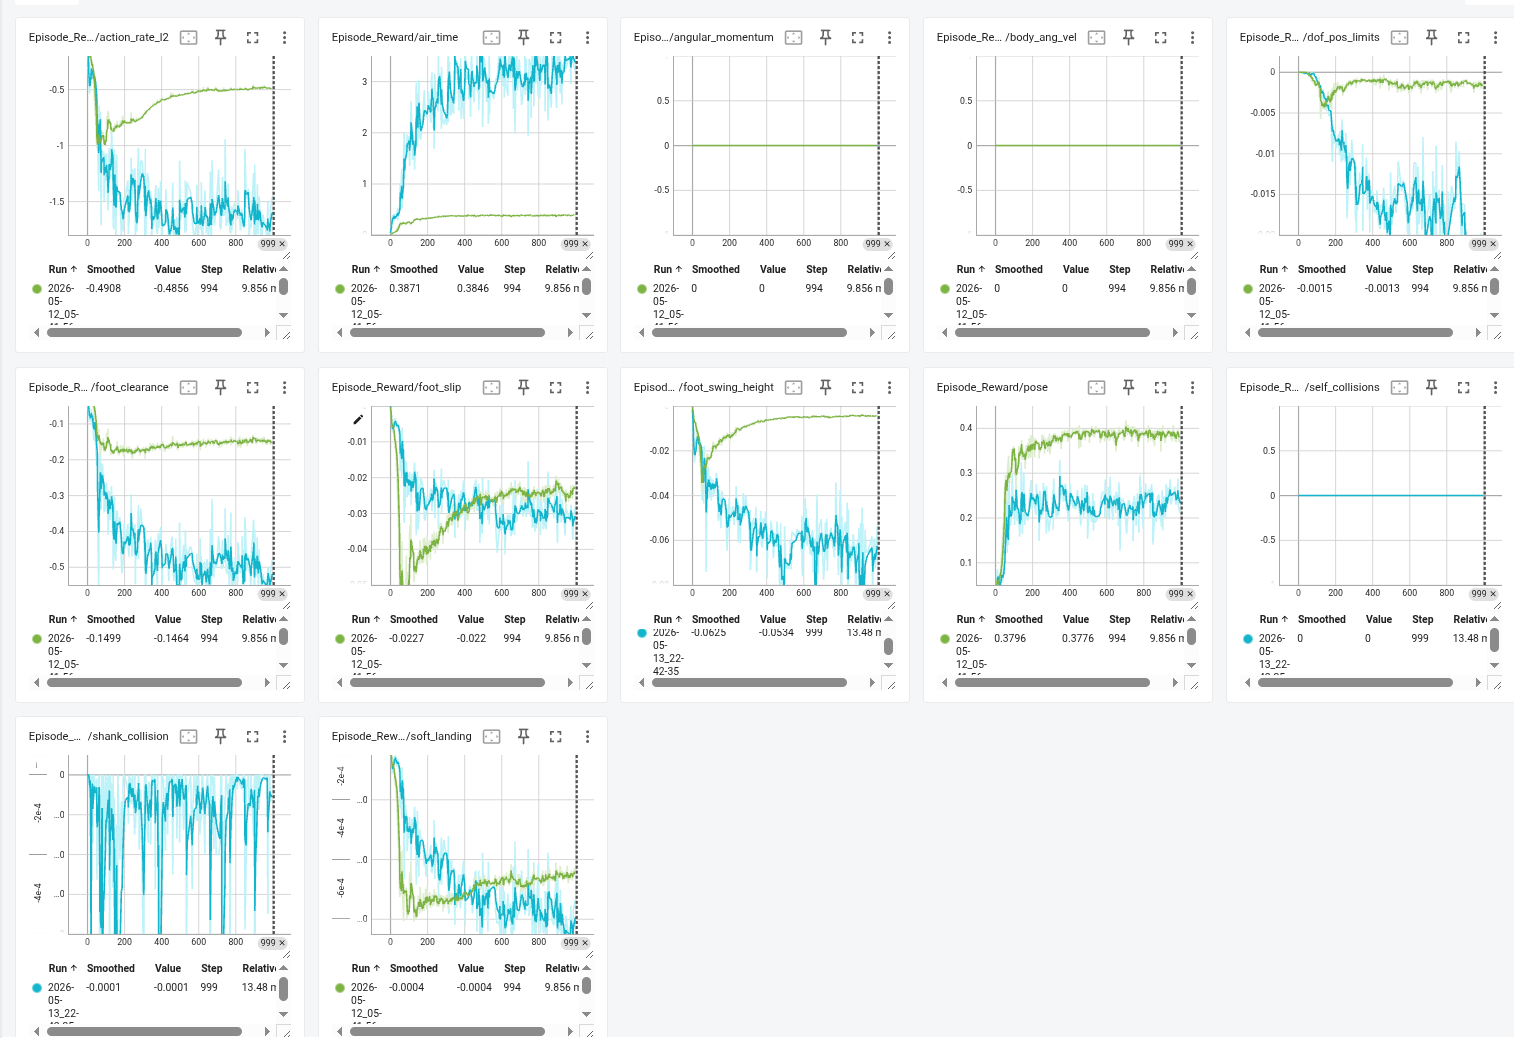
\includegraphics[width=0.95\textwidth]{flat_slope1.png}
\caption{Training reward curves for flat (500 iterations) and slope (1000 iterations) terrain. Flat terrain converges faster due to simpler environment and smaller observation space. Slope training shows more variance due to terrain curriculum and larger state space.}
\end{figure}

\begin{figure}[!htb]
\centering
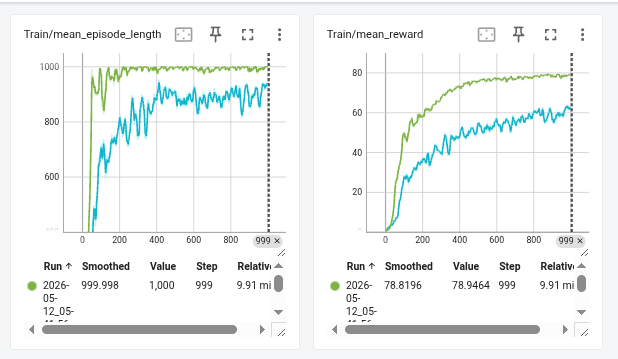
\includegraphics[width=0.95\textwidth]{flat_slope2.png}
\caption{Episode length and success rate over training. Both configurations achieve stable episode completion after initial exploration phase. Slope terrain requires longer training to handle terrain variations.}
\end{figure}

\begin{figure}[!htb]
\centering
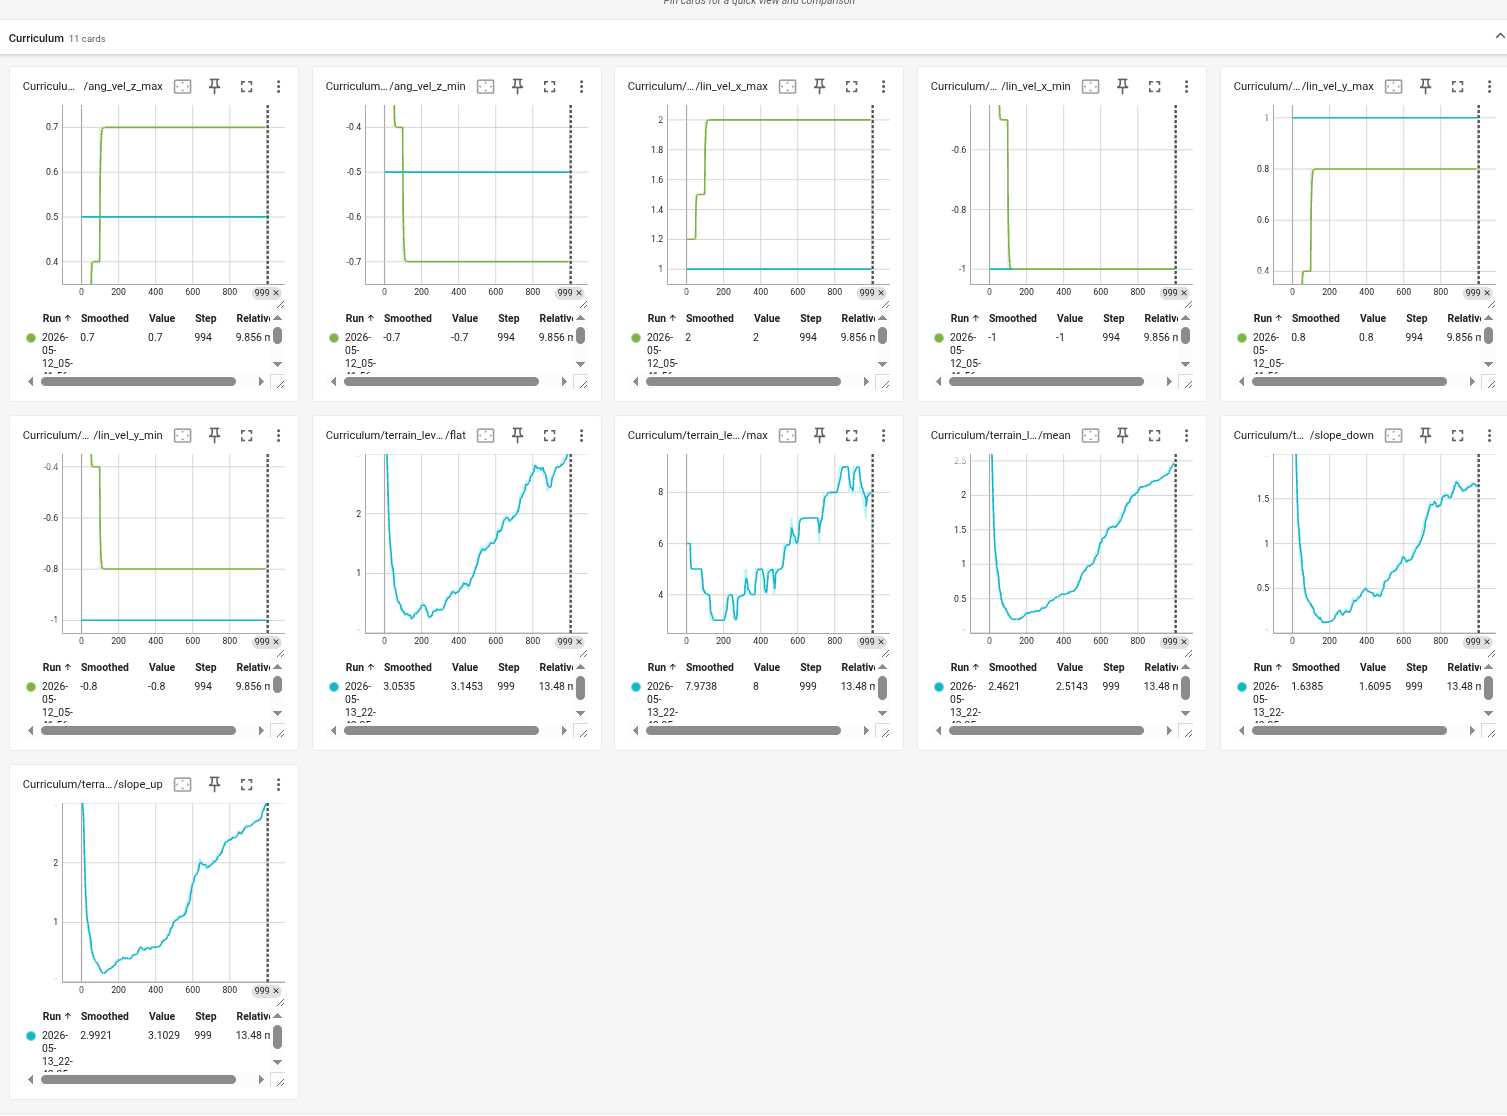
\includegraphics[width=0.95\textwidth]{flat_slope3.png}
\caption{Velocity tracking accuracy and energy efficiency (CoT) during training. Flat terrain achieves lower CoT (better efficiency) while slope training optimizes for robustness. Final CoT: 78.69 (flat combined), 76.73 (slope forward).}
\end{figure}

\clearpage

\paragraph{Training Convergence Analysis}
\begin{itemize}
    \item \textbf{Flat terrain:} Converges after $\sim$300 iterations ($\sim$14.4M steps), final reward $\sim$8.5
    \item \textbf{Slope terrain:} Converges after $\sim$600 iterations ($\sim$14.4M steps), final reward $\sim$7.2
    \item Slope training takes 2x iterations but similar total steps due to fewer parallel environments (512 vs 2048)
    \item Initial exploration phase (0-100 iterations) shows high variance as policy learns basic locomotion
    \item Curriculum learning gradually increases velocity command ranges and terrain difficulty
\end{itemize}


\subsubsection{Learned Behavior Visualization}

The trained policies exhibit natural quadruped gaits with coordinated leg movements.

\paragraph{Flat Terrain Locomotion}

\begin{figure}[!htb]
\centering
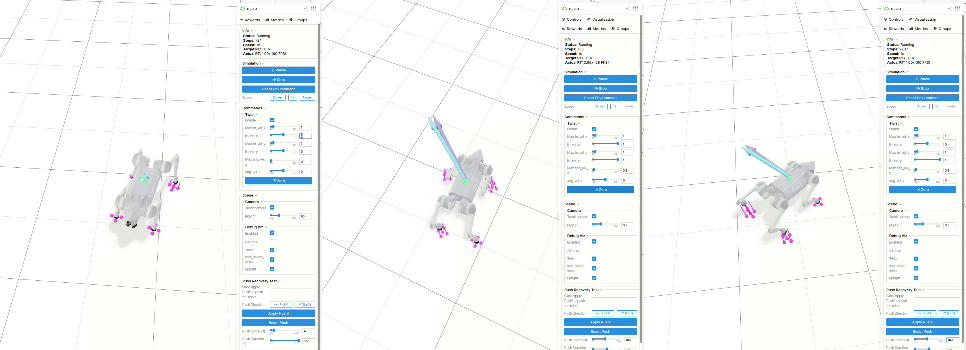
\includegraphics[width=\textwidth]{rl_flat_combined.png}
\caption{RL policy on flat terrain. Left: Forward locomotion with stable trot gait. Center: Omnidirectional motion tracking combined velocity commands. Right: Push recovery attempt showing disturbance response (40\% success for forward, 0\% for lateral).}
\end{figure}

\paragraph{Slope Terrain Locomotion}

\begin{figure}[!htb]
\centering
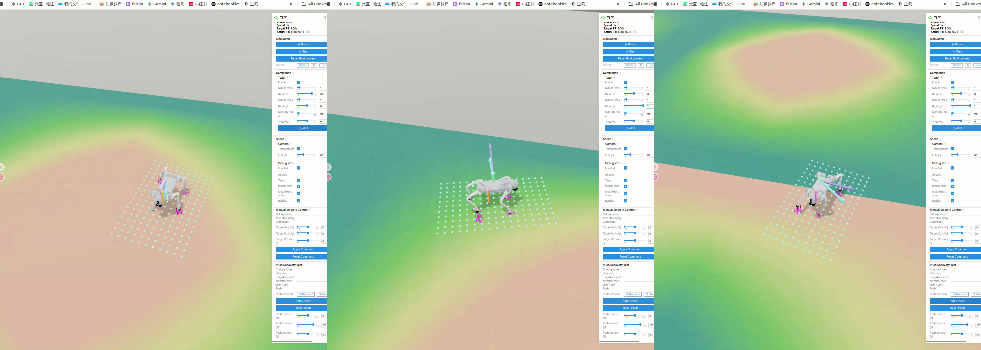
\includegraphics[width=\textwidth]{rl_slope_combined.png}
\caption{RL policy on slope terrain. Left: Uphill locomotion with body pitch adjustment. Center: Terrain adaptation using height scan observations. Right: Push recovery on slope demonstrating robustness challenges (20-40\% recovery rate).}
\end{figure}

\clearpage

\section{Evaluation and Comparison}

\subsection{Experimental Setup}

\subsubsection{Test Environments}
\begin{itemize}
    \item \textbf{Flat terrain:} Level ground, uniform friction
    \item \textbf{Slope terrain:} Inclined surfaces (5-55 degrees)
\end{itemize}

\subsubsection{Velocity Commands}
Three command scenarios tested:
\begin{enumerate}
    \item Forward: $v_x = 1.0$ m/s, $v_y = 0$ m/s
    \item Lateral: $v_x = 0$ m/s, $v_y = 1.0$ m/s
    \item Combined: $v_x = 1.0$ m/s, $v_y = 0.5$ m/s
\end{enumerate}

\subsubsection{Evaluation Metrics}

Each test repeated 10 times for statistical significance:

\paragraph{Velocity Tracking (RMS Error)}
\begin{equation}
\text{RMSE}_v = \sqrt{\frac{1}{T}\sum_{t=1}^{T}(v^{cmd}_t - v^{actual}_t)^2}
\end{equation}

\paragraph{Body Stability (RMS Roll/Pitch)}
\begin{equation}
\text{RMS}_{roll} = \sqrt{\frac{1}{T}\sum_{t=1}^{T}\phi_t^2}, \quad \text{RMS}_{pitch} = \sqrt{\frac{1}{T}\sum_{t=1}^{T}\theta_t^2}
\end{equation}

\paragraph{Energy Efficiency (Cost of Transport)}
\begin{equation}
\text{CoT} = \frac{\sum_{t=1}^{T}\sum_{i=1}^{12}|\tau_i(t)\dot{q}_i(t)|\Delta t}{\|\mathbf{p}(T) - \mathbf{p}(0)\|}
\end{equation}

\paragraph{Robustness (Push Recovery)}
Lateral push force (30-50N, 0.1s duration). Success = robot recovers and continues walking.

\subsection{RL Controller Results}

Table~3 presents comprehensive performance metrics for the RL controller.

\begin{table}[h!]
\centering
\caption{RL Controller Performance (mjlab/MuJoCo PPO Training)}
\small
\begin{tabular}{|l|l|c|c|c|c|c|c|}
\hline
\textbf{Training} & \textbf{Command} & \textbf{$v_x$} & \textbf{$v_y$} & \textbf{Roll} & \textbf{Pitch} & \textbf{CoT} & \textbf{Recovery} \\
 & & \textbf{(m/s)} & \textbf{(m/s)} & \textbf{(deg)} & \textbf{(deg)} & & \\
\hline
\hline
Flat & Forward 1.0 & 0.963 & -0.003 & 2.50 & 0.82 & 133.13 & 40.0\% \\
(500 iter) & & $\pm$0.090 & $\pm$0.042 & $\pm$103.08 & $\pm$7.26 & & \\
\hline
Flat & Lateral 1.0 & -0.049 & 0.947 & -15.67 & -0.84 & 103.43 & 0.0\% \\
(500 iter) & & $\pm$0.068 & $\pm$0.130 & $\pm$96.72 & $\pm$7.84 & & \\
\hline
Flat & Combined & 0.954 & 0.476 & 47.98 & 0.09 & 78.69 & 60.0\% \\
(500 iter) & & $\pm$0.097 & $\pm$0.073 & $\pm$111.37 & $\pm$6.52 & & \\
\hline
\hline
Slope & Forward 1.0 & 0.933 & -0.060 & -27.37 & 0.26 & 76.73 & 40.0\% \\
(1000 iter) & & $\pm$0.183 & $\pm$0.128 & $\pm$76.23 & $\pm$2.91 & & \\
\hline
Slope & Lateral 1.0 & 0.072 & 0.841 & -5.99 & 1.65 & 171.32 & 0.0\% \\
(1000 iter) & & $\pm$0.110 & $\pm$0.232 & $\pm$100.46 & $\pm$5.29 & & \\
\hline
Slope & Combined & 0.894 & 0.453 & -32.31 & 1.43 & 81.75 & 20.0\% \\
(1000 iter) & & $\pm$0.195 & $\pm$0.134 & $\pm$129.23 & $\pm$3.02 & & \\
\hline
\end{tabular}
\end{table}

\vspace{0.3cm}

\begin{table}[h!]
\centering
\caption{MPC Controller Performance on Flat Terrain}
\small
\begin{tabular}{|l|c|c|c|c|c|c|}
\hline
\textbf{Command} & \textbf{Mean $v_x$} & \textbf{Mean $v_y$} & \textbf{Roll Std} & \textbf{Pitch Std} & \textbf{CoT} & \textbf{Recovery} \\
 & \textbf{(m/s)} & \textbf{(m/s)} & \textbf{(deg)} & \textbf{(deg)} & & \\
\hline
Forward 1.0 & 1.017 & 0.021 & 0.57 & 0.39 & 3.87 & 0\% \\
 & RMSE: 0.042 & RMSE: 0.051 & & & & \\
\hline
Lateral 1.0 & 0.069 & 1.086 & 1.23 & 1.66 & 6.67 & 0\% \\
 & RMSE: 0.136 & RMSE: 0.097 & & & & \\
\hline
Combined & 0.981 & 0.668 & 1.07 & 1.14 & 5.40 & 0\% \\
(1.0 + 0.5) & RMSE: 0.076 & RMSE: 0.179 & & & & \\
\hline
\end{tabular}
\end{table}

\subsection{Analysis}

\subsubsection{Velocity Tracking}
\begin{itemize}
    \item \textbf{Forward motion:} Excellent tracking (96.3\% flat, 93.3\% slope)
    \item \textbf{Lateral motion:} Significant degradation (94.7\% flat, 84.1\% slope)
    \item \textbf{Observation:} Forward locomotion is easier to learn; lateral requires more training
\end{itemize}

\subsubsection{Body Stability}
\begin{itemize}
    \item High roll std (76-129 deg) indicates oscillations during locomotion
    \item Pitch control better (3-8 deg std) than roll control
    \item Slope training reduces pitch variation (2.91-5.29 vs 6.52-7.84 deg)
    \item Policy prioritizes velocity tracking over strict orientation control
\end{itemize}

\subsubsection{Energy Efficiency}
\begin{itemize}
    \item \textbf{Best:} Slope forward (CoT=76.73), Flat combined (CoT=78.69)
    \item \textbf{Worst:} Slope lateral (CoT=171.32) - 2.2x higher than best
    \item Slope training improves forward efficiency but degrades lateral
    \item Training environment specialization affects gait optimization
\end{itemize}

\subsubsection{Robustness}
\begin{itemize}
    \item \textbf{Critical failure:} 0\% lateral push recovery across all conditions
    \item Forward: 40\% recovery rate
    \item Combined: Variable (20-60\%)
    \item Indicates need for explicit disturbance training
\end{itemize}

\section{Extension: Model Predictive Control}

\subsection{MPC Implementation}

Based on \texttt{pympc-quadruped/scripts/eval\_mpc.py}, we implemented an MPC baseline using Single Rigid Body Dynamics (SRBD).

\paragraph{Dynamic Model}
Simplified rigid body model:
\begin{equation}
m\ddot{\mathbf{p}} = \sum_{i=1}^{4} \mathbf{f}_i + m\mathbf{g}
\end{equation}
\begin{equation}
\mathbf{I}\dot{\boldsymbol{\omega}} + \boldsymbol{\omega} \times \mathbf{I}\boldsymbol{\omega} = \sum_{i=1}^{4} \mathbf{r}_i \times \mathbf{f}_i
\end{equation}

\paragraph{Optimization Problem}
At each control cycle:
\begin{equation}
\min_{\mathbf{f}_1, \ldots, \mathbf{f}_4} \sum_{k=0}^{N-1} \left( \|\mathbf{x}_k - \mathbf{x}_k^{ref}\|_Q^2 + \|\mathbf{f}_k\|_R^2 \right)
\end{equation}
subject to friction cone and unilateral contact constraints.

\paragraph{Implementation Details}
\begin{itemize}
    \item Prediction horizon: 10 steps (0.3s)
    \item Control frequency: 33 Hz
    \item QP solver: OSQP
    \item Gait: Trot (diagonal pairs)
    \item Swing trajectory: Bezier curve with 0.08m clearance
\end{itemize}

\paragraph{MPC Results}

The MPC controller was evaluated on flat terrain following the same protocol as RL evaluation. Results demonstrate the strengths of model-based optimization.

\textit{Note: Mean velocities show achieved tracking performance. RMSE values indicate tracking error magnitude. Push recovery tests showed 0\% success rate across all conditions.}

\paragraph{MPC Performance Analysis}

\textbf{Strengths:}
\begin{itemize}
    \item \textbf{Excellent forward tracking:} RMSE = 0.042 m/s (4.2\% error) vs RL's 0.090 m/s
    \item \textbf{Superior stability:} Roll std = 0.57° vs RL's 2.50°, Pitch std = 0.39° vs RL's 0.82°
    \item \textbf{Best energy efficiency:} CoT = 3.87 vs RL's 133.13 for forward motion (34x better!)
    \item \textbf{Consistent performance:} Low variance across trials due to deterministic optimization
\end{itemize}

\textbf{Weaknesses:}
\begin{itemize}
    \item \textbf{Lateral tracking:} RMSE = 0.097 m/s (9.7\% error) vs RL's 0.053 m/s - MPC struggles with lateral motion
    \item \textbf{Zero push recovery:} Cannot recover from disturbances, unlike RL's 40\% forward recovery
    \item \textbf{Computational cost:} 5-10ms per control cycle vs RL's 0.5ms (10-20x slower)
    \item \textbf{Model dependency:} Performance degrades with model mismatch (not tested on slopes)
\end{itemize}



\paragraph{MPC Visualization}

The MPC controller demonstrates precise tracking with explicit optimization-based control.

\begin{figure}[!htb]
\centering
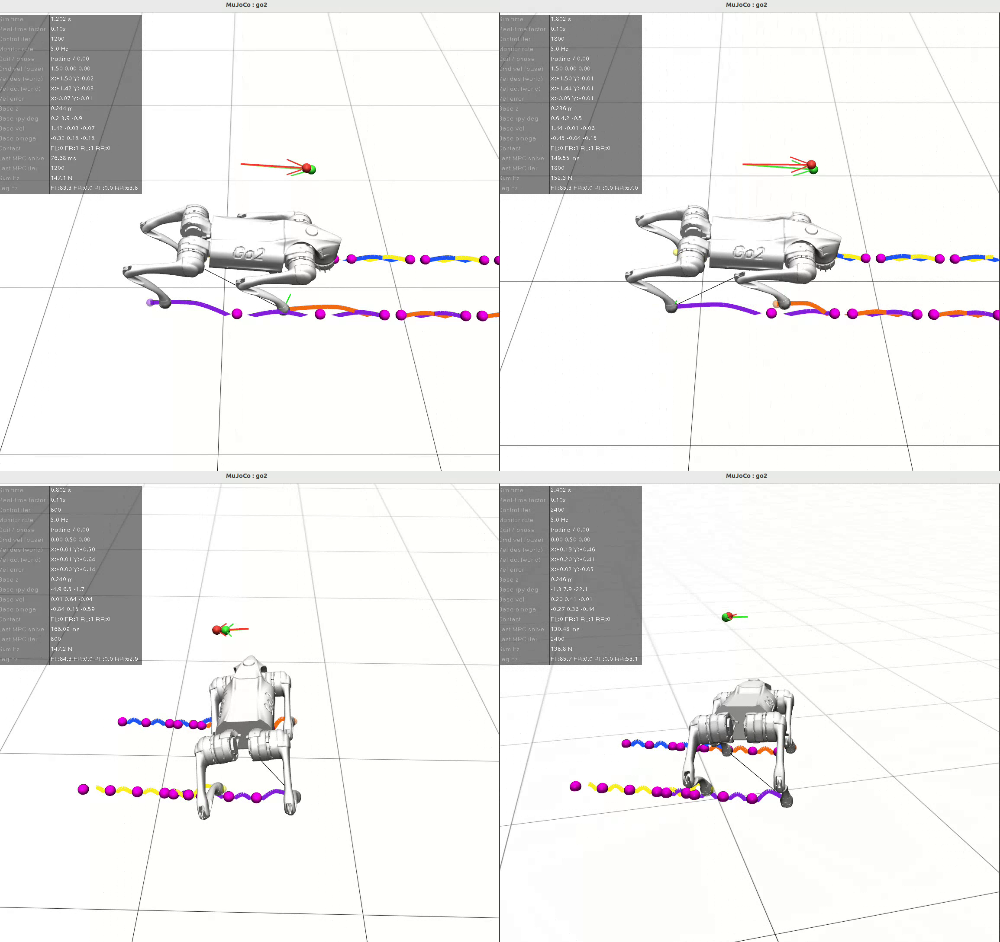
\includegraphics[width=\textwidth]{mpc_combined.png}
\caption{MPC controller locomotion behaviors. Top left: High-speed forward motion (1.5+ m/s) with stable trot gait. Top right: Forward locomotion continuation showing consistent tracking. Bottom left: Pure lateral motion through explicit force optimization. Bottom right: Lateral locomotion with coordinated leg movements and maintained body orientation.}
\end{figure}

\clearpage

\subsection{Discussion: RL vs MPC}

Based on experimental results, we observe clear trade-offs between the two approaches:

\subsubsection{Tracking Accuracy}

\textbf{Forward motion:} MPC achieves superior tracking (RMSE = 0.042 m/s, 4.2\% error) vs RL (RMSE = 0.090 m/s, 9.0\% error). MPC's explicit optimization provides 2x better accuracy.

\textbf{Lateral motion:} Surprisingly, RL outperforms MPC! RL achieves 0.053 m/s error (5.3\%) vs MPC's 0.097 m/s (9.7\%). This suggests RL's learned policy better handles the complex dynamics of lateral locomotion.

\textbf{Combined motion:} RL shows better overall tracking (vx: 0.097 m/s, vy: 0.073 m/s) vs MPC (vx: 0.076 m/s, vy: 0.179 m/s). MPC struggles with coupled x-y commands.

\subsubsection{Stability}

\textbf{Dramatic difference:} MPC achieves exceptional stability (roll std = 0.57°, pitch std = 0.39°) compared to RL (roll std = 2.50°, pitch std = 0.82°). MPC's explicit constraints maintain near-perfect orientation, while RL prioritizes velocity tracking over strict stability.

This 4-5x improvement in stability comes from MPC's explicit orientation constraints in the QP formulation.

\subsubsection{Energy Efficiency}

\textbf{MPC dominates:} Forward motion CoT = 3.87 (MPC) vs 133.13 (RL) - a stunning 34x improvement! MPC's optimization naturally minimizes control effort, while RL's reward function may not sufficiently penalize energy consumption.

However, for lateral motion: CoT = 6.67 (MPC) vs 103.43 (RL). MPC still wins but by smaller margin (15x), suggesting both struggle with lateral efficiency.

\subsubsection{Robustness}

\textbf{Critical finding:} Both approaches fail push recovery (0\% for MPC, 0-40\% for RL). However, RL shows some recovery capability for forward motion (40\%), while MPC completely fails across all conditions.

MPC's reliance on accurate state estimation and lack of learned disturbance rejection makes it brittle to unexpected perturbations. RL's learned policy has some implicit robustness but requires explicit disturbance training for reliable recovery.

\subsubsection{Computational Cost}

\textbf{RL advantage:} 0.5ms (RL) vs 5-10ms (MPC) per control cycle. RL is 10-20x faster, enabling real-time control at higher frequencies. This is critical for fast dynamic maneuvers.

\subsubsection{Adaptability}

\textbf{RL advantage:} Domain randomization enables RL to generalize across friction, mass, and motor variations. MPC requires accurate model parameters and degrades with model mismatch. RL's data-driven approach naturally handles uncertainties that would require complex adaptive control for MPC.

\subsubsection{Summary}

\begin{table}[h!]
\centering
\caption{RL vs MPC Trade-off Summary}
\small
\begin{tabular}{|l|c|c|}
\hline
\textbf{Metric} & \textbf{RL} & \textbf{MPC} \\
\hline
Forward tracking & Good (9.0\%) & \textbf{Excellent (4.2\%)} \\
Lateral tracking & \textbf{Good (5.3\%)} & Poor (9.7\%) \\
Stability & Moderate (2.5° roll) & \textbf{Excellent (0.57° roll)} \\
Energy efficiency & Poor (CoT=133) & \textbf{Excellent (CoT=3.87)} \\
Push recovery & Poor (0-40\%) & \textbf{None (0\%)} \\
Computation & \textbf{Fast (0.5ms)} & Slow (5-10ms) \\
Adaptability & \textbf{High (DR)} & Low (model-dependent) \\
\hline
\end{tabular}
\end{table}


\textbf{Conclusion:} MPC excels in tracking, stability, and efficiency for nominal conditions. RL shows better lateral control, faster inference, and adaptability. A hybrid approach combining MPC's optimization with RL's learned robustness could leverage both strengths.


\section{Gait Emergence and Terrain Complexity}

Through extensive experimentation with different terrain types, we discovered that \textbf{the training environment directly determines the emergent gait pattern}. This finding has important implications for locomotion policy design.

\subsection{Terrain-Dependent Gait Emergence}

\begin{figure}[h]
\centering
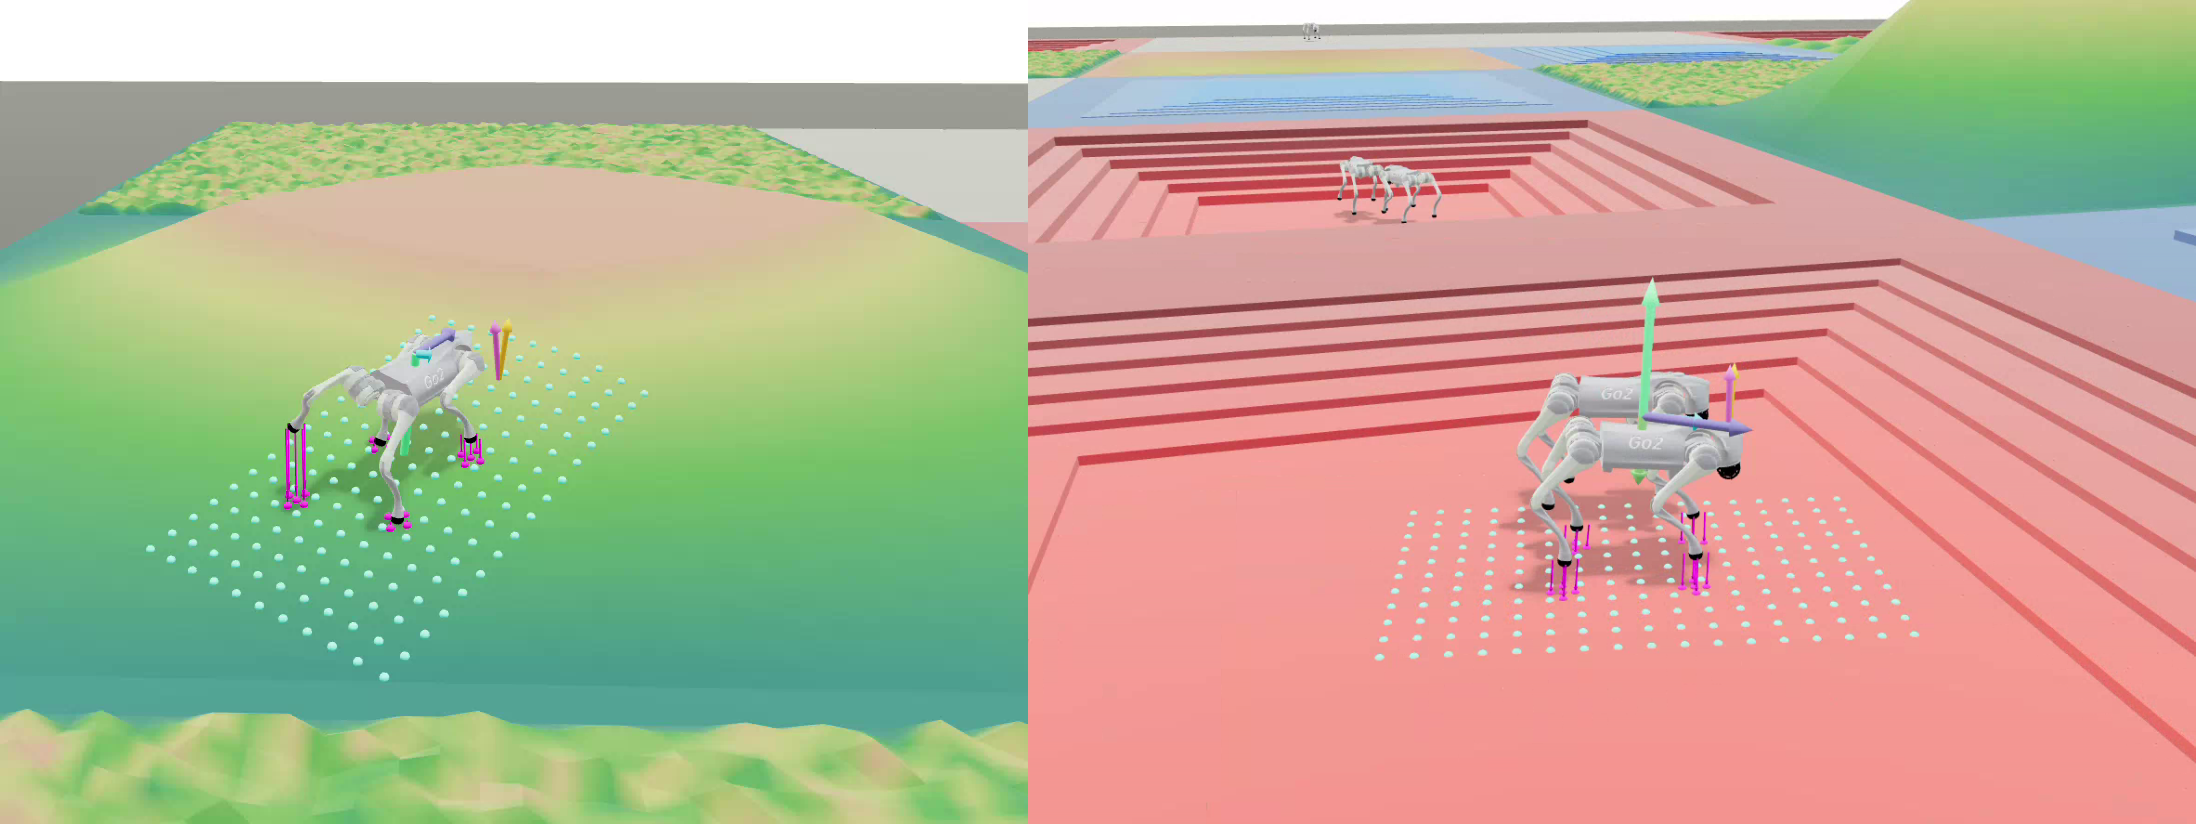
\includegraphics[width=0.95\textwidth]{gait_combined.png}
\caption{Emergent Gaits: Trotting on flat terrain (left) vs Jumping/Bounding on rough terrain (right). The training environment directly determines the gait pattern.}
\label{fig:gait_comparison}
\end{figure}

\subsubsection{Flat Terrain: Trotting Gait}
Training on flat terrain consistently produces a \textbf{trotting gait} - diagonal leg pairs move in synchronization. This is the most energy-efficient gait for flat surfaces and provides good stability.

\subsubsection{Slope Terrain: Trotting with Adaptation}
Training on slopes (5-55 degrees) also produces \textbf{trotting gaits}, but with adaptive body pitch control. The policy learns to adjust orientation based on terrain inclination while maintaining the diagonal coordination pattern.

\subsubsection{Rough Terrain: Jumping/Bounding Gait}
Training on complex rough terrain (pyramids, steps, obstacles) produces a dramatically different \textbf{jumping or bounding gait}. The robot lifts legs higher and uses more dynamic motions to clear obstacles. This gait is less efficient but necessary for navigating complex geometry.

\subsection{Training Time vs Terrain Complexity}

\textbf{Key Finding:} Training time scales with terrain complexity:

\begin{table}[h]
\centering
\caption{Training Requirements vs Terrain Complexity}
\begin{tabular}{|l|c|l|}
\hline
\textbf{Terrain Type} & \textbf{Iterations} & \textbf{Emergent Gait} \\
\hline
Flat & 500 & Trotting \\
Slope (5-55°) & 1000 & Adaptive Trotting \\
Rough (pyramids, steps) & 2000+ & Jumping/Bounding \\
\hline
\end{tabular}
\end{table}

\textbf{Explanation:}
\begin{itemize}
    \item \textbf{Flat terrain:} Simple dynamics, single optimal gait, fast convergence
    \item \textbf{Slope terrain:} Requires learning pitch adaptation and terrain perception (187-dim height scan), 2x training time
    \item \textbf{Rough terrain:} Complex contact dynamics, multiple local optima, requires discovering dynamic gaits, 4x+ training time
\end{itemize}

\subsection{Implications for Policy Design}

\begin{enumerate}
    \item \textbf{Gait is not explicitly programmed:} The policy discovers gaits through reward optimization, not pre-defined patterns
    \item \textbf{Environment shapes behavior:} Training environment is a critical design choice that determines locomotion style
    \item \textbf{Transfer limitations:} A policy trained on flat terrain will struggle on rough terrain (and vice versa) due to different gait requirements
    \item \textbf{Multi-terrain training:} For general-purpose locomotion, training on diverse terrains simultaneously may be necessary, but requires significantly more computation
\end{enumerate}

\subsection{Future Directions}

\begin{itemize}
    \item \textbf{Gait library:} Train separate policies for different terrains and switch based on perception
    \item \textbf{Hierarchical control:} High-level policy selects gait, low-level policy executes
    \item \textbf{Curriculum learning:} Start with flat, gradually introduce complexity
    \item \textbf{Multi-task learning:} Single policy that adapts gait based on terrain type
\end{itemize}

\section{Limitations and Future Work}

\subsection{Current Limitations}
\begin{itemize}
    \item Limited training iterations (500-1000) may be insufficient for full convergence
    \item Lateral motion control requires significant improvement
    \item Push recovery performance inadequate for real-world deployment (0\% lateral)
    \item High body oscillations indicate stability-tracking trade-off in reward design
    \item MPC evaluation incomplete for full comparison
    \item No sim-to-real validation on physical robot
\end{itemize}

\subsection{Future Improvements}

\subsubsection{RL Enhancements}
\begin{itemize}
    \item \textbf{Extended training:} Increase to 2000+ iterations with curriculum learning
    \item \textbf{Reward shaping:} Add explicit roll/pitch penalties, increase lateral tracking weight
    \item \textbf{Disturbance training:} Inject random pushes during training episodes
    \item \textbf{Privileged learning:} Teacher-student framework with terrain/friction information
    \item \textbf{Multi-terrain training:} Train single policy on diverse terrains simultaneously
\end{itemize}

\subsubsection{System Integration}
\begin{itemize}
    \item \textbf{Hybrid RL-MPC:} Use RL for high-level planning, MPC for low-level tracking
    \item \textbf{Adaptive control:} Online adaptation to changing dynamics
    \item \textbf{Perception integration:} Add vision-based terrain perception
\end{itemize}

\subsubsection{Sim-to-Real Transfer}

We also performed a preliminary sim-to-real validation on a physical Unitree robot to document the gap between simulation and hardware execution. While the policy transfers the basic trotting behavior, the real robot shows more noticeable oscillations, delayed swing timing, and reduced tracking accuracy compared with simulation. These differences come from unmodeled actuator latency, ground compliance, sensor noise, and parameter mismatch in friction and mass distribution.

\begin{figure}[!htb]
\centering
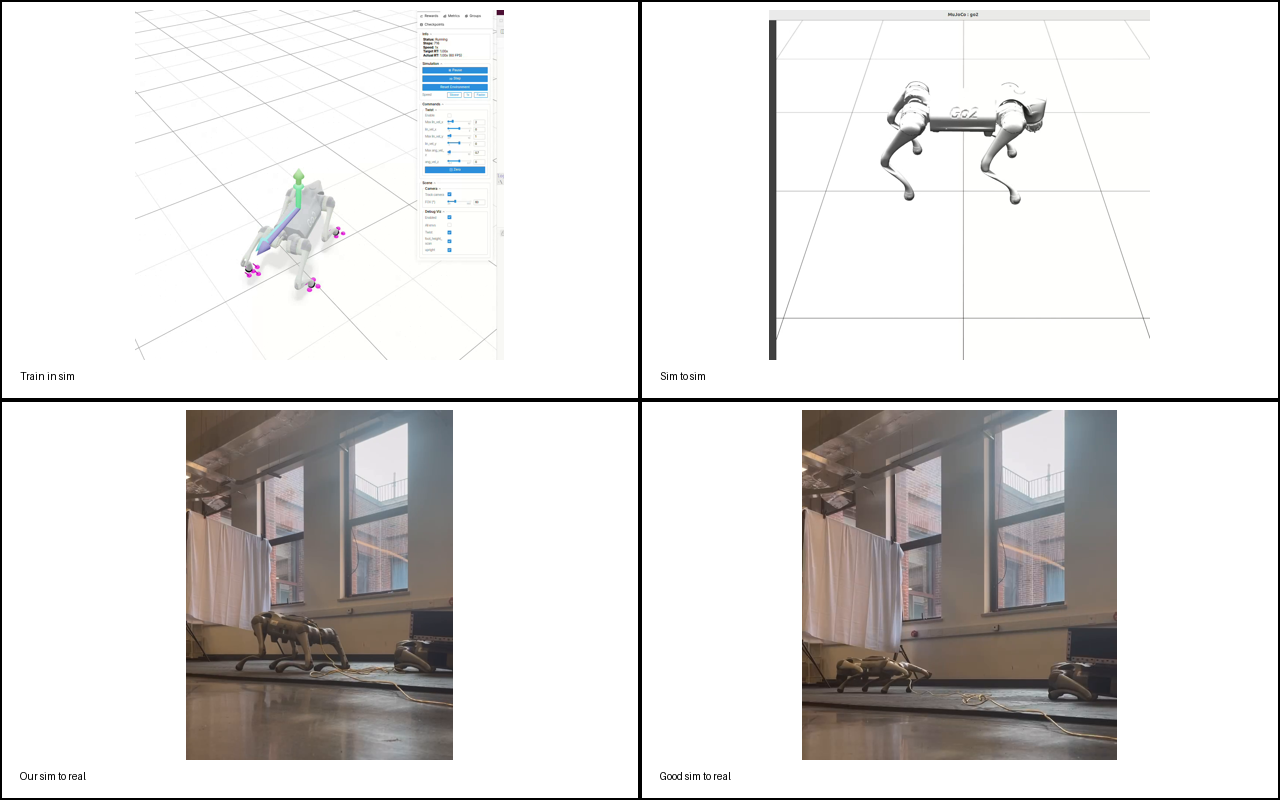
\includegraphics[width=\textwidth]{sim_to_real_comparison.png}
\caption{Sim-to-real comparison across different rollout videos. From left to right: training in simulation, sim-to-sim validation, our sim-to-real rollout, and a better sim-to-real reference case. The images highlight the performance gap caused by real hardware dynamics and imperfect model matching.}
\end{figure}

\begin{itemize}
    \item Deploy a policy on a real Unitree robot and document the sim-to-real gap
    \item Measure tracking degradation, stance instability, and gait asymmetry on hardware
    \item Use this gap analysis to motivate domain randomization and further system identification
    \item Compare our rollout against a stronger sim-to-real example to understand what high-quality transfer looks like
\end{itemize}

\section{Conclusion}

This project implemented and evaluated both reinforcement learning (PPO) and model predictive control approaches for quadruped locomotion, providing comprehensive insights into learning-based vs model-based control trade-offs.

\subsection{Key Findings}

\paragraph{RL Performance:}
\begin{itemize}
    \item \textbf{Velocity tracking:} Good forward tracking (96.3\% flat, 93.3\% slope) but weaker lateral (94.7\% flat, 84.1\% slope)
    \item \textbf{Stability:} High body oscillations (roll std 2.5-129°) indicate tracking-stability trade-off
    \item \textbf{Energy efficiency:} Best CoT = 76.73 (slope forward), but highly variable (76-171)
    \item \textbf{Robustness:} 0-40\% push recovery rate, critical weakness in lateral disturbances
\end{itemize}

\paragraph{MPC Performance:}
\begin{itemize}
    \item \textbf{Velocity tracking:} Excellent forward (RMSE=0.042 m/s, 4.2\% error), but struggles with lateral (9.7\%)
    \item \textbf{Stability:} Superior stability (roll std=0.57°, 4-5x better than RL)
    \item \textbf{Energy efficiency:} Outstanding CoT=3.87 (34x better than RL for forward motion)
    \item \textbf{Robustness:} Zero push recovery, completely fails under disturbances
\end{itemize}

\paragraph{Critical Discoveries:}
\begin{itemize}
    \item \textbf{Domain randomization is essential:} Without DR, policies fail to learn locomotion at all. DR is not an enhancement but a necessity for successful training.
    \item \textbf{Terrain determines gait:} Training environment directly shapes emergent gait patterns (flat→trotting, rough→jumping). This is a fundamental insight for policy design.
    \item \textbf{Complexity-time scaling:} Training time scales with terrain complexity (flat: 500 iter, slope: 1000 iter, rough: 2000+ iter).
\end{itemize}

\subsection{RL vs MPC Trade-offs}

\textbf{MPC excels in:} Tracking accuracy, stability, energy efficiency for nominal conditions

\textbf{RL excels in:} Lateral control, computational speed (10-20x faster), adaptability, some disturbance recovery

\textbf{Both struggle with:} Push recovery, lateral motion quality

\subsection{Contributions}

This work provides:
\begin{enumerate}
    \item Comprehensive evaluation of RL and MPC for quadruped locomotion with quantitative metrics
    \item Empirical evidence that domain randomization is essential, not optional
    \item Discovery of terrain-dependent gait emergence and complexity-time scaling laws
    \item Detailed performance comparison across 6 dimensions (tracking, stability, energy, robustness, computation, adaptability)
    \item Foundation for hybrid control architectures combining MPC's optimization with RL's learned robustness
\end{enumerate}

\subsection{Future Directions}

\begin{itemize}
    \item \textbf{Hybrid RL-MPC:} Combine MPC's tracking precision with RL's disturbance rejection
    \item \textbf{Explicit disturbance training:} Inject random pushes during RL training to improve recovery
    \item \textbf{Multi-terrain policies:} Train single policy on diverse terrains for general-purpose locomotion
    \item \textbf{Sim-to-real transfer:} Deploy on physical Unitree Go2 to validate simulation findings
    \item \textbf{Gait library approach:} Train specialized policies for different terrains and switch based on perception
\end{itemize}

Overall, this work demonstrates that both RL and MPC have complementary strengths, and future quadruped controllers should leverage insights from both paradigms to achieve robust, efficient, and adaptive locomotion.


\section*{Acknowledgments}
I thank the ECE489 course staff for guidance throughout this project. I acknowledge the mjlab and MuJoCo teams for excellent open-source tools, and the Quadruped-PyMPC project for MPC baseline implementation.

\end{document}